\documentclass[a4paper, 12pt]{report}

\usepackage[french]{babel}
\usepackage[latin1]{inputenc}
\usepackage[T1]{fontenc}

\usepackage[french]{varioref}
\usepackage[french]{minitoc}

\usepackage{geometry}
\usepackage{fancyhdr}
\usepackage{graphicx}

\usepackage{latexsym}
\usepackage{amsmath}
\usepackage{amssymb}

\usepackage{listings}
\lstset{language=Java, frame=single, mathescape=true, showspaces=false}
\lstset{numbers=left, numberstyle=\tiny, stepnumber=2, numbersep=5pt,
  basicstyle=\small, frameround=tttf, frame=tRBl}

\geometry{vmargin=3cm, hmargin=3cm}

\title{\huge{Une interface graphique pour Vaucanson}\\
  Rapport de stage\\
\vspace{5cm}
\small{R�sum�:
Le but de ce stage est de produire un prototype interface graphique
pour Vaucanson. En partant d'un prototype existant, dont il faudra
principalement r�organiser la structure, un autre prototype sera
produit. On esp�re cette fois atteindre un niveau de qualit�
permettant sa diffusion. Une documentation sera aussi produite,
facilitant ainsi les �volutions futures du projet.}
}

\author{Guillaume \bsc{Leroi}\\ UID: 18147}

\lhead{Rapport de stage}
\chead{}
\rhead{ENST - INFRES}

\geometry{vmargin=3cm, hmargin=3cm}
\linespread{1.3}
\pagestyle{empty}


\begin{document}
\maketitle
\thispagestyle{empty}
\newpage

\doparttoc
\dominitoc
\tableofcontents
\thispagestyle{empty}
\newpage

\pagestyle{fancy}
\setcounter{page}{1}
\chapter{Introduction}
Vaucanson est une plateforme logicielle d�di�e � la manipulation
d'automates et de transducteurs. D�velopp� au LRDE en partenariat avec
Jacques Sakarovitch (ENST) et Sylvain Lombardy (LIAFA), Vaucanson est
une biblioth�que g�n�rique permettant d'utiliser et d'�crire des
algorithmes pour une grande vari�t� d'automates.

A la fin de l'�t� 2006, la version 1.0 de Vaucanson est sortie
proposant une suite d'outils en ligne de commande comme interface
utilisateur. La plateforme Vaucanson est d�sormais utilisable sans
mettre en oeuvre de programmation.

Par ailleurs, un prototype d'interface graphique pour Vaucanson a �t�
r�alis� 2004 par Louis-No�l Pouchet. Le but de ce stage est de
produire, � partir de ce prototype, une version toujours exp�rimentale
mais diffusable et document�e.

A terme, l'interface graphique (que l'on appellera VGI, pour l'instant)
fournira un moyen d'utiliser Vaucanson plus facilement
qu'en utilisant l'API et avec plus de souplesse que le TAF-KIT. Ce
stage se place dans une vision � long terme, et ne vise pas � rendre un
produit totalement fini.  Le logiciel produit devra permettre de
visualiser des automates simples, de modifier sa forme et son
apparence graphique et d'appliquer les algorithmes propos�s par le
TAF-KIT � ces automates.  Une grande partie de tout cela est d�j�
accompli par le prototype, cependant une r�organisation du code, la
production d'une documentation d�veloppeur reste � faire, afin de
faciliter les am�liorations futures.

\paragraph{Inter�t personnel}

Ce stage me permet de d�couvrir un projet annexe � la biblioth�que
elle-m�me, par ailleurs le premier prototype a �t� �crit en
Java. Ainsi l'occasion m'ait donn� de d�couvrir ce langage, les
biblioth�ques associ�es et ses environnements de d�veloppement.

Par ailleurs, la r�alisation de ce logiciel permettra peut-�tre de
d�couvrir des erreurs dans Vaucanson ou le TAF-KIT, qui pourront �tre
rapport�es � l'�quipe Vaucanson et supprim�es.

\paragraph{D�roulement du stage}

Apr�s avoir �t� re�u et pr�sent� � l'administration de l'ENST, une
s�rie de r�union ont �t� planifi� avec M. Sakarovitch, mon ma�tre de
stage, et Louis-No�l Pouchet, pour mettre au point ensemble une
mod�lisation coh�rente du projet. En parall�le � ces r�unions, je
devais d�couvrir et me familiariser avec le code de VGI.

Puis, la mise en oeuvre des d�cisions prises lors des r�unions a
commenc�. Dans un premier temps, quelques bugs simples ont �t�
corrig�s, puis le module XML a �t� mis � jour en fonction de la
derni�re sp�cification parue.
Le code a subi une mise � jour g�n�ral pour utiliser la derni�re
version de la biblioth�que JGraph, ainsi que quelques corrections de
bugs.
Finalement, les modification n�cessaires pour que VGI se conforme � la
mod�lisation d�cid�e ont �t� entreprises.

Une fois que le remodelage du projet fut suffisamment avanc�, un d�but
de documentation d�veloppeur fut �crite, elle prit forme au fur et �
mesure de l'�tat d'avancement et des modifications fa�tes au projet.

\paragraph{Particularit� de ce stage}

On notera que la partie ``pr�sentation de l'entreprise'' n'est pas
pr�sente. En effet, bien que ce stage ait lieu � l'ENST, celle-ci n'a
pas de lien avec le stage. Ainsi on ne trouvera pas dans ce
rapport de consid�rations sur l'int�gration de mon travail dans
l'ENST.


\chapter{Travail effectu�}

\section{Cahier des charges}


\subsection{But g�n�ral}

Le but de ce stage est de produire, � partir d'un prototype existant,
une version toujours exp�rimentale mais diffusable et document�e.  Le
logiciel produit devra permettre de visualiser des automates simples,
d'�diter ses propri�t�s g�om�triques et graphiques et d'appliquer les
algorithmes propos�s par le TAF-KIT � ces automates.

La documentation utilisateur permettra de d�couvrir et d'expliquer les
fonctionnalit�s du logiciel. Cette documentation existant d�j� depuis
le premier prototype, il faudra la mettre � jour.

Une documentation d�veloppeur est n�cessaire. Elle devra pr�senter la
structure du projet, pr�senter les diff�rents modules. C'est � dire
expliquer leur utilit�, leur fonctionnement et donner des indications
sur l'emplacement de certains calculs.


\subsection{R�sultats � obtenir}

Le prototype existant �tait d�j� � une stade avanc�, il permettait de:
\begin{itemize}
\item afficher un automates � partir d'un fichier XML
\item modifier cet automate et ces diff�rentes propri�t�s
\item appliquer des algorithmes � ces automates
\end{itemize}

\vspace{0.3cm}

\subsubsection{R�organisation du code}

L'un des principaux buts de ce stage est d'organiser le projet en
quatre modules distincts et ind�pendants. Cette mod�lisation comporte:

\begin{itemize}
\item le module XML: il permet de charger et sauvegarder des automates
  au format XML (existait d�j� dans le prototype).
\item le module g�om�trique: il g�re la manipulation des valeurs
  g�om�triques, comme les coordonn�es d'un �tat, la forme d'une
  transition, toutes informations se rattachant � la ``forme g�n�ral''
  de l'automate.
\item le module graphique: il g�re la manipulation des propri�t�s
  graphiques de l'automate, tel que l'emplacement d'un label sur sa
  transition, la couleur d'un �tat, l'�paisseur d'une transition.
\item le module d'affichage: ce module traduit les propri�t�s
  g�om�triques et graphiques pour JGraph.
\end{itemize}

Les modules g�om�trique et graphique doivent fournir des valeurs par
d�faut pour les propri�t�s qu'ils g�rent.
Les quatre modules forme les diff�rentes �tapes par lesquelles un
automate passera.

\begin{itemize}
\item XML: A partir du fichier XML, on construit un objet VJGraph, qui
  repr�sent� notre automate.
\item Puis il passe dans le module g�om�trique. Si certains �l�ments
  ne disposent pas de propri�t�s g�om�triques, celles-ci sont ajout�es
  avec les valeurs par d�faut.
\item De m�me pour le module graphique et les propri�t�s associ�es.
\item Finalement le module d'affichage traduit les propri�t�s
  pr�c�dentes pour JGraph.
\end{itemize}

\subsubsection{Corrections mineures}

Le premi�re version de l'interface graphique pour Vaucanson (VGI) a
�t� �crite en 2004, depuis le projet Vaucanson a connu plusieurs
modifications que VGI n'a pas suivi. Il faudra donc, un premier temps,
mettre � jour VGI en fonction de Vaucanson 1.0.

\vspace{0.3cm}

En particulier:
\begin{itemize}
\item le format XML a quelque peu chang�
\item les algorithmes �taient appliqu�s grace � l'utilisation
  d'ex�cutables sp�ciaux, il serait int�ressant de les remplacer par
  ceux du TAF-KIT.
\end{itemize}

\vspace{0.3cm}

De plus, le prototype utilise JGraph pour afficher et manipuler le
graphe de l'automate. Cette biblioth�que ayant �volu� depuis
2004, il faudra donc mettre � jour le prototype pour qu'il puisse
utiliser la derni�re version de JGraph disponible.

Notons que la n�cessit� d'utiliser la derni�re version de JGraph
disponible est apparu eu cours du stage, et ne semblait pas n�cessaire
au d�but.

Outre les mises � jour, certaines fonctionnalit�s n�cessitent des
modifications.\\
Le prototype de d�part permet de sauvegarder les propri�t�s
g�om�triques et graphiques du graphe. Mais les unit�s utilis�es ne
sont pas toujours celles d�sir�es. Par ailleurs, certaines propri�t�s
d�finies dans le format XML ne sont pas utilis�es, ou mal utilis�es.

\vspace{0.3cm}

On souhaiterait que:
\begin{itemize}
\item la position d'un �tat soit exprim�e dans une unit� ind�pendante,
  pas en pixel.
\item les unit�s des angles soit des degr�s et non des radians.
\item le label d'une transition soit positionn� selon un pourcentage
  (ou 0\% repr�sente le d�but de la transition et 100\% l'extr�mit�
  fl�ch�e de la transition) et non pas en utilisant des coordonn�es
  absolues.
\item l'op�ration de centrage de l'automate ne modifie les coordonn�es
  des �tats de l'automate, mais ``d�place'' la fen�tre pour que
  l'automate y soit centr�.
\end{itemize}

\subsubsection{Documentation}

Le manuel utilisateur existe d�j�, il a �t� �crit par Pouchet lors de
son stage en 2004. Celui-ci d�taille l'utilisation de l'interface
graphique, c'est � dire comment charger et sauvegarder un automate,
comment en cr�er un nouveau, utiliser les algorithmes et changer les
diff�rentes propri�t�s. Ce manuel �tant complet, il ne n�cessitera
probablement pas de modifications.\\

La documentation d�veloppeur est quand � elle quasi inexistante.
Certaines parties du code sont document�es mais elles sont rares et
rarement au format Javadoc ou Doxygen. Le code en fait ne demande que
peu de documentation, il est g�n�ralement tr�s simple. Cependant un
document expliquant la structure du projet, l'utilit� des diff�rents
modules et les classes qui les composent, faciliterait la prise en
main du code pour les �tudiants qui seraient amen�s a y travailler.

\section{Compte-rendu d'activit�}

\subsection{Conception}

Avec l'aide de mon ma�tre de stage et de Louis-Noel Pouchet, une
mod�lisation a �t� d�cid�. Cette mod�lisation est bas� sur les
diff�rentes �tapes que se d�tachent quand on analyse notre mani�re de
dessiner un automate.

Trois �tapes se d�tachent en particulier:
\begin{enumerate}
\item On d�cide de la forme de l'automate, c'est � dire on place les
  �tats, on d�cide de la forme de transition, l'emplacement des labels.
\item Puis on d�cide de son apparence, certains �tats doivent �tre
  color�s, l'�paisseur des transitions.
\item Le rendu final, ou l'affichage � l'�cran.
\end{enumerate}

Dans le cas de notre logiciel, l'automate est contenu dans un fichier
XML, il faut donc un module dont la tache est de lire se fichier et de
cr�er un objet manipulable par le reste du programme.

Par ailleurs, l'affichage est g�r� par JGraph. Il n'est donc pas
n�cessaire d'�crire un module d'affichage, mais plutot un module
charg� de traduire les diff�rentes propri�t�s graphiques et
g�om�triques de l'automate.

Au final, la mod�lisation pr�sent�e par la figure \ref{fig:mod}, a �t�
obtenue.

\begin{figure}[h]
  \centering
  %%FIXME: faire l'uml des quatre packages.
  \caption{Mod�lisation g�n�ral du projet}
  \label{fig:mod}
\end{figure}


\subsection{Modules}

\subsubsection{XML}

Le module XML utilis� est celui d�j� pr�sent dans le premier
prototype. Quelques modifications sont cependant n�cessaire pour que
le module soit � jour par rapport � l'�tat actuel du format XML.

Ces mises � jour consistent globalement � changer le nom de certains
attributs, et d'utiliser les modules Geometry et Drawing pour extraire
les donn�es � stocker dans le fichier XML.


\subsubsection{Module g�om�trique et graphique}

Les modules g�om�triques et graphiques sont en tout point
semblables. Ils ne diff�rent que par l'ensemble des propri�t�s qu'ils
g�rent.

Le module Geometry permet la manipulation des propri�t�s g�om�triques
de l'automate, et en particulier celles de ses �tats et
transitions. Chaque �tat ou transition poss�de deux tables
associatives contenant leurs propri�t�s g�om�triques et graphiques.

Les valeurs contenues par ces tables sont extraites et ins�r�es gr�ce
� la classe GeometryProperties qui fournit un ensemble de m�thodes
statiques, ainsi que des valeurs par d�faut pour chaque propri�t�.
Les types des valeurs �tant assez vari�s (entier, chaine de caract�re,
�num�ration), toutes les donn�es sont stock�es sous forme de chaine de
caract�re dans la table associative.

Ainsi d'une part, leur sauvegarde au format XML est facilit� et
d'autre part la classe GeometryProperties se charge de fournir les
donn�es vers les types concrets. Ainsi on pourra dans le futur
modifier la mani�re dont les propri�t�s sont stock�s en m�moire sans
modifier trop de code. Il suffira d'adapter les diff�rentes m�thodes
statiques de la classe GeometryProperties.

La figure \ref{fig:geo} pr�sentent quelques exemples de m�thodes que
l'on peut trouver dans la classe GeometryProperties.

\begin{figure}[h]
\begin{lstlisting}
public final static String TRANSITIONTYPE = "transitionType";
public static void setTransitionType(Transition e, String type)
{
  Map geometry = e.geometry_get();

  if (type != null || type.equals(LINE) || type.equals(ARCL) ||
      type.equals(ARCR) || type.equals(CURVE))
       geometry.put(TRANSITIONTYPE, type);
  else
       geometry.put(TRANSITIONTYPE, TRANSITIONTYPEDEFAULT);
}

public static String getTransitionType(Transition e)
{
  Map geometry = e.geometry_get();
  String type = (String) geometry.get(TRANSITIONTYPE);
  return type;
}

// Values for transitionType
public final static String LINE = "line";
public final static String ARCL = "arcL";
public final static String ARCR = "arcR";
public final static String CURVE = "curve";
public final static String TRANSITIONTYPEDEFAULT = LINE;
\end{lstlisting}

  \caption{Extrait de code de la classe GeometryProperties}
  \label{fig:geo}
\end{figure}

Une fois les classes GeometryProperties et DrawingProperties cr��es,
il a fallu mettre � jour l'ensemble du code pour qu'il utilise ces
m�thodes. Ainsi le module XML et l'ensemble des classes g�rant
l'interaction avec l'utilisateur ont �t� adapt�s pour utiliser ces
m�thodes.


\subsubsection{Module d'affichage}

Le module d'affichage est compos� d'un ensemble de classe charg�es de
fournir � JGraph des indications sur comment dessiner le graphe de
l'automate, ou qui parfois �tendent le comportement de JGraph en
prenant en charge elles m�me certaines parties du dessin.

Ainsi dans ce module on trouvera les classes:
\begin{itemize}
\item Router: � partir des informations g�om�triques d'une transition,
  principalement sa forme (ligne, arc), cette classe fournit une suite
  de points par lesquelles le trac� de la transition doit passer.
\item StateView: cette classe prend en charge l'affichage d'un �tat.
\item TransitionView: cette classe ne g�re que l'affichage d'un label
  associ� � une transition. Cependant, elle pourrait a l'avenir
  prendre en charge l'affichage de la transition.
\end{itemize}




\end{document}


\chapter{Conclusion}
Le but de ce stage �tait de produire une interface graphique pour
Vaucanson � partir d'un prototype existant. Le logiciel produit serait
toujours un prototype mais l�g�rement plus �volu�, et surtout ayant
subi une r�organisation de son code. Une documentation devait aussi
�tre �crite.\\

Dans ce rapport, nous avons d�taill� la nouvelle mod�lisation du
projet, plus modulaire, qui rend le logiciel plus �volutif. En
particulier cette nouvelle mod�lisation simplifie grandement les
modifications portant l'ajout de nouvelles propri�t�s g�om�triques et
graphiques.
Cette mod�lisation a �t� mise au point au cours de plusieurs r�unions
avec M. Sakarovitch et M. Pouchet, en �tudiant la mani�re dont l'on
dessine un automate � la main et par comparaison avec l'exp�rience
acquise lors de la r�alisation du premier prototype.\\

De plus, avec la documentation d�veloppeur produite, la prise en main
du code par de futures stagiaires sera plus ais�e. La documentation
donne des indications sur la mod�lisation, l'utilit� et le
fonctionnement des diff�rents modules. Elle identifie aussi
l'emplacement de certains calculs importants pour la mise en forme de
l'automate.\\

Le prototype produit lors de ce stage comporte aussi la correction de
plusieurs bugs, un interface plus agr�able pour rapporter le r�sultat
de certains algorithmes � l'utilisateur, et une mise � jour g�n�ral du
code par rapport au �volution de Vaucanson, du format XML et de JGraph
depuis le prototype du stage pr�c�dent.\\

On notera que m�me si les objectifs de ce stage sont
globalement atteints, l'interface graphique n�cessitera encore de
nombreuses am�liorations avant d'�tre largement diffusable. En
particulier au niveau de l'ergonomie de l'interface. Il faudra faire
face aussi � des probl�mes de rapidit� et de qualit� du rendu
graphique, car bien que ce dernier �l�ment soit correct, il n'a pas
�t� test� avec des automates poss�dant de nombreux �tats.

Finalement, Vaucanson poss�de un embryon d'interface graphique. Et
cette interface graphique permettra � plus long terme d'utiliser la
plateforme Vaucanson plus facilement que par l'API C++ et avec plus de
souplesse que le TAF-KIT.


\part{Annexes}
\parttoc
\newpage
%%\listoffigures
\newpage
\setcounter{chapter}{0}
\chapter{Mod�lisation}

\begin{figure}[h]
  \centering
  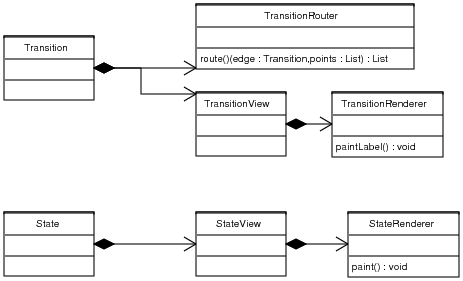
\includegraphics[width=16cm]{img/Affichage.png}
  \caption{Fonctionnement du module d'affichage}
  \label{fig:affichage}
\end{figure}

\begin{figure}[h]
  \centering
  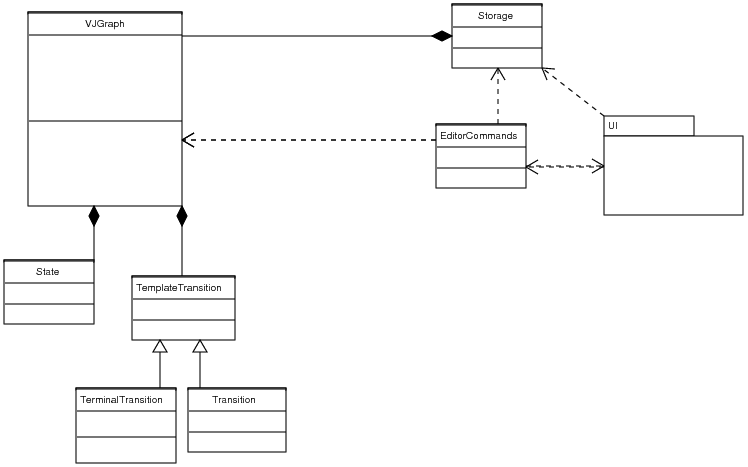
\includegraphics[width=16cm]{img/Overview.png}
  \caption{Vue g�n�rale du programme}
  \label{fig:overview}
\end{figure}

\begin{figure}[h]
  \centering
  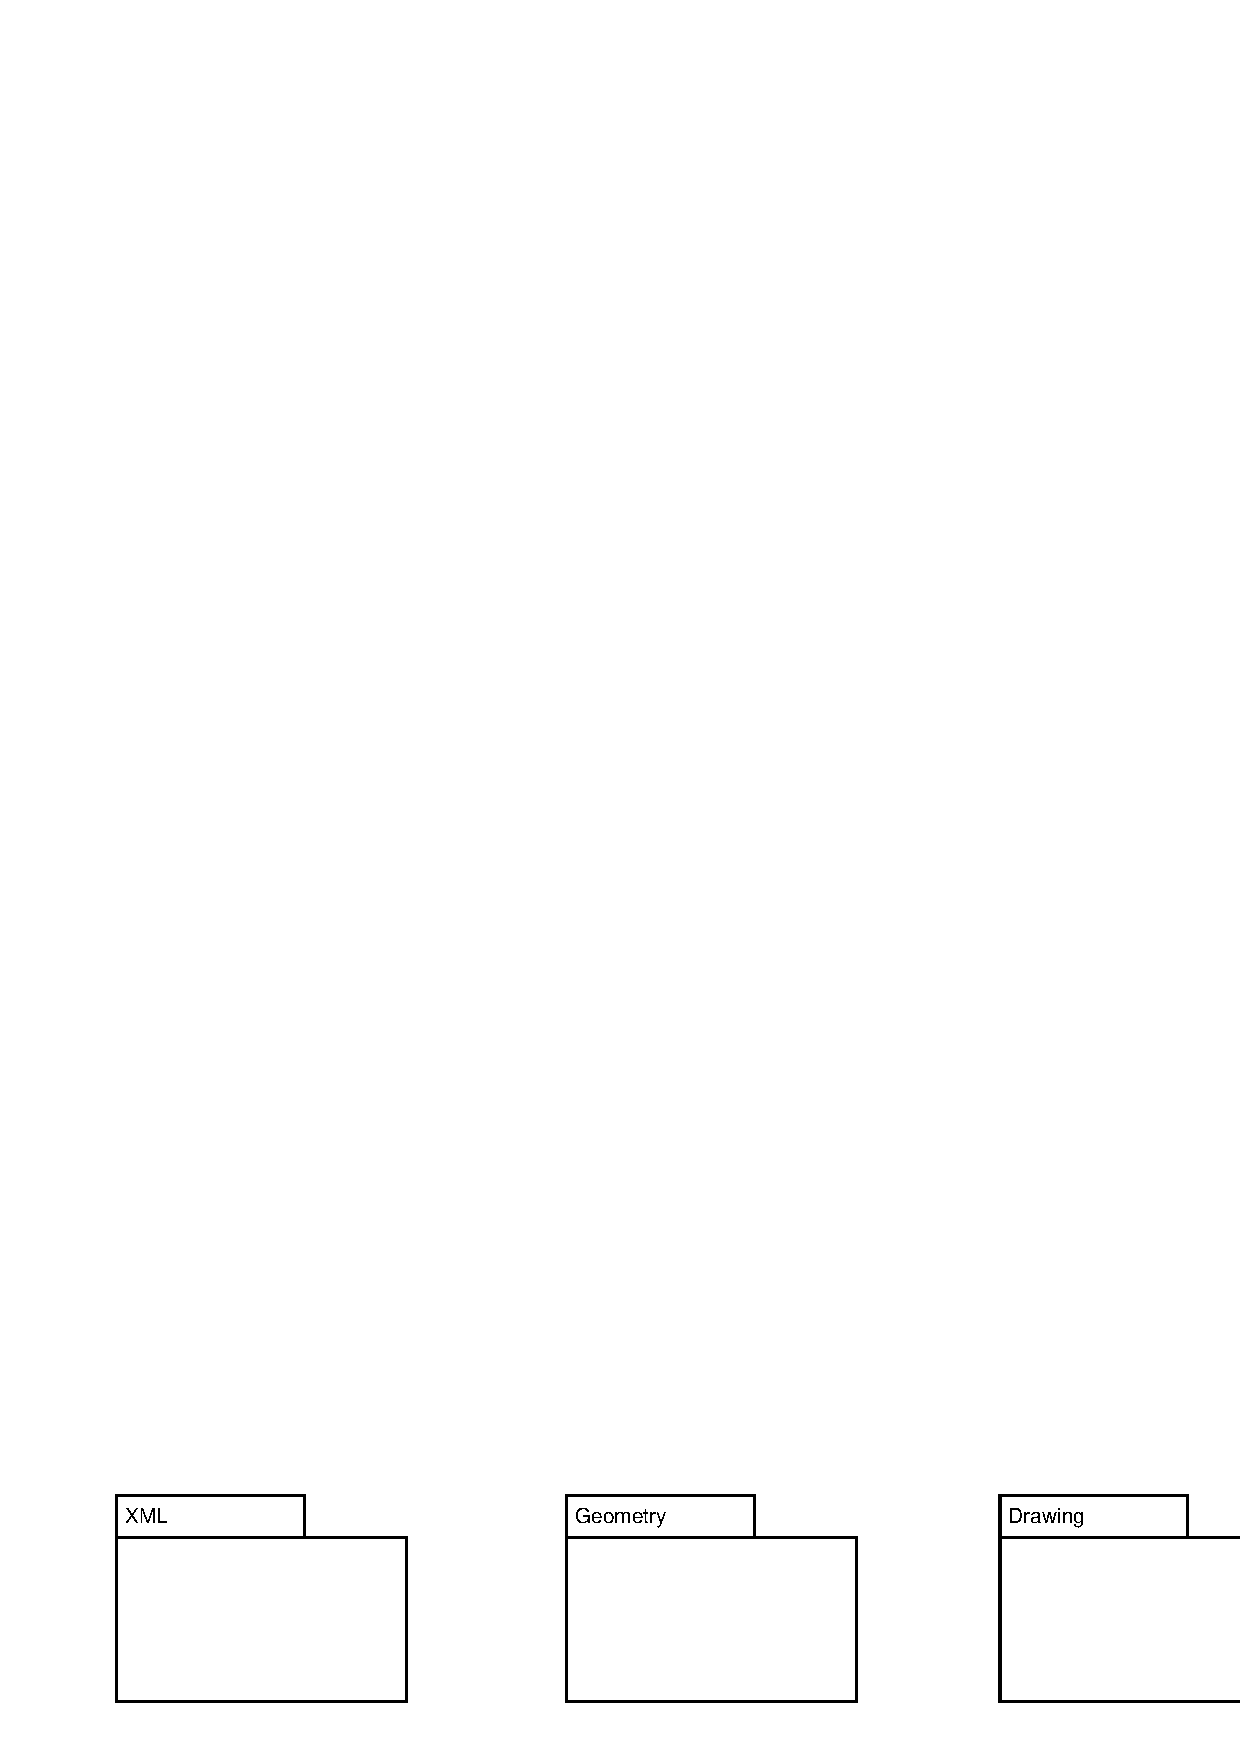
\includegraphics[width=16cm]{img/Packages.png}
  \caption{Mod�lisation des packages}
\end{figure}

\begin{figure}[h]
  \centering
  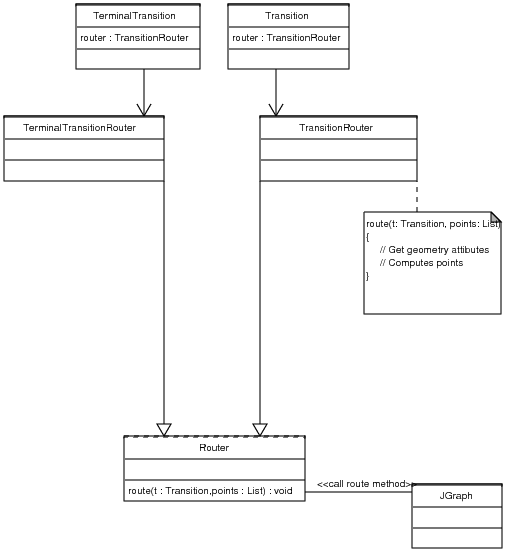
\includegraphics[width=16cm]{img/routing.png}
  \caption{Module d'affichage: Routage des transitions}
  \label{fig:router}
\end{figure}

\chapter{Screenshots}

\begin{figure}[h]
  \centering
  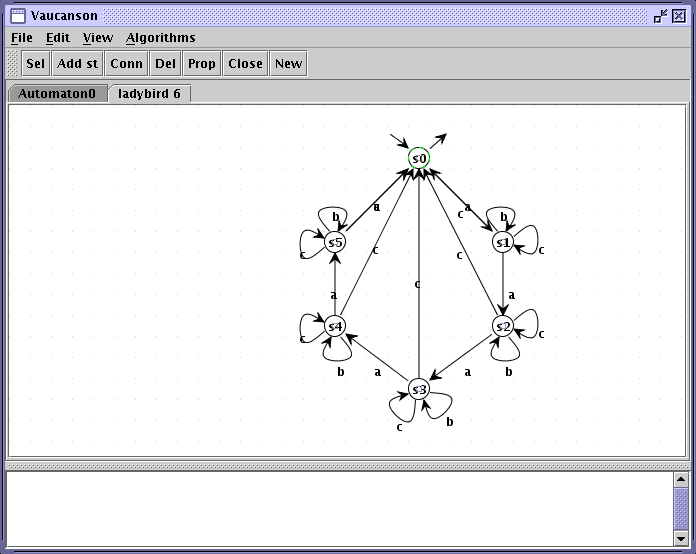
\includegraphics[width=12cm]{img/ui.png}
  \caption{Fen�tre principale}
  \label{fig:ui}
\end{figure}

\begin{figure}[h]
  \centering
  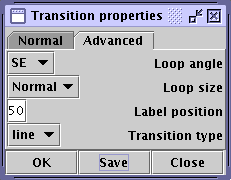
\includegraphics[width=6cm]{img/transition.png}
  \caption{Fen�tre des propri�t�s d'une transition}
  \label{fig:ui_prop}
\end{figure}

\begin{figure}[h]
  \centering
  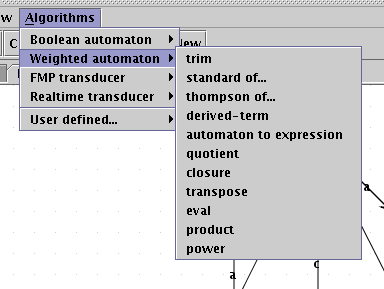
\includegraphics[width=8cm]{img/menu.png}
  \caption{Le menu des algorithmes disponibles}
  \label{fig:algo_menu}
\end{figure}

\chapter{Documentation}
\label{doc}
\section{Modules}

In this section, the directory hierarchy will be described. Some
informations about what does a module will be given too.

Now, VGI is composed of two packages: vgi and vgitoolkit.
\begin{itemize}
\item The vgi package contains the user interface, the code that manage the
interaction between the user, the graphical interface and vgitoolkit.

\item The vgitoolkit contains the geometry and drawing modules, a module
extending the graph class of JGraph to meet our requirements, and some
code translating geometry and drawing properties to JGraph
instructions.
\end{itemize}


\subsection[src/vgi]{VGI package}

In this directory can be found all classes for the user interface, and
some related tools.

\begin{itemize}
\item VGI.java: contains the main function, and creates the editor
  main window.

\item Storage.java: manages informations between the user interface
  and JGraph object. In it exist functions which allow us to find the
  corresponding JGraph object of a panel, or the corresponding XML
  file of a panel. If a algorithm is call by the user, this class
  selects the correct binary following the automaton type.

\item EditorCommands.java: contains utility functions like creating a
  new graph, state or transition. It performs action user required on
  JGraph object.

\item IO.java: contains utility code to call executables, give them
  some input and send output back to VGI.

\item StateProperties.java and TransitionProperties.java: contain the
  user interface for editing geometry and drawing properties of states
  and transitions.
\end{itemize}


\subsection[src/vgitoolkit/vaucanson/vgitoolkit]{VGIToolkit package}

This package contains our graph model for JGraph, utilities for
loading and saving to the XML format. It contains too the geometry and
drawing modules.

\subsubsection{VJGraph}

VJGraph extends the JGraph class to meet our requirements, i.e add
some functionalities to the graph class (JGraph) to become an
automaton class (VJGraph).

Three classes have been created: VJGraph, State and Transition.
Each class contain a geometry and drawing maps.
VJGraph contains informations on the automaton type.
State contains informations on its final and initial transitions.
Transition contains informations on its label and how to display it
following the type of the automaton.

\subsubsection{Geometry module}

The Geometry module is composed of the following classes:
GeometryProperties, GeometricUtilities, and all layout classes.

\paragraph{Geometry Properties:}

This class defines functions to retrieve and set geometry properties
from State or Transition. It enforces the correctness of the given
value and defines some defaults values if nothing was define in the
XML file.

\paragraph{Layouts:}

The goal of layout classes is to provide a nice embedding to the graph.

Layout classes are use to set the location of each states of a
graph. A layout is applied by calling its \emph{apply} method. A
utility class, LayoutTemplate, which all layouts extend, is given. It
defines standard methods for retrieving selected states.

For the time being, layouts only define position of states. But place
has been left so they can modify the geometry properties of
transitions too. TemplateLayout provide a default implementation of a
method which set geometry properties of transitions.

Finally, LayoutTemplate provides a special method to translate the
geometry properties of a set of states to JGraph instructions.

\paragraph{GeometricUtilities:}

This class contains some utility functions, as finding a free angle on
a state for a transition, bezier calculations and so on.


\subsubsection{Drawing module}

\paragraph{Drawing Properties:}

This class is just the same than GeometryProperties but for drawing
properties.

\subsubsection{XML}

Three classes are defined XMLConverter, XMLReader and XMLWriter.

\begin{itemize}
\item XMLConverter: converts a VJGraph object to DOM representation
  and vice-versa.
\item XMLReader: abstraction for reading from a file or string.
\item XMLWriter: abstraction for writing to a file or string.
\end{itemize}


\subsubsection{Translation to JGraph}

As said before the translation of geometry properties of states to
JGraph is done after applying a layout.
The rest of the properties, either geometric or drawing properties,
are translated in different classes. Here is a list of them, each
entry describes what it translates:

\begin{itemize}
\item Router: transition's geometric properties are translated in
  classes TransitionRouter, LoopRouter and TerminalTransitionRouter
  (see Figure \ref{diaroute}).
\item StateView: this class translates drawing properties of states.
\item TransitionView: here is translated drawing AND geometric
  properties of transitions.
\end{itemize}

\begin{figure}[h]
  \centering
  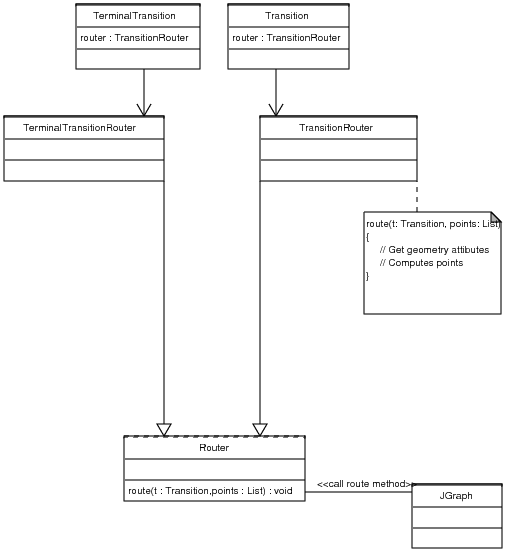
\includegraphics[width=16cm, height=20cm]{img/routing.png}
  \caption{Translation of geometric properties of transitions}
  \label{diaroute}
\end{figure}




\end{document}




\end{document}
